\label{key}\documentclass[letterpaper, 12pt,oneside]{article}
\usepackage{amsmath}
\usepackage{graphicx}
\usepackage{xcolor}
\graphicspath{{Imagenes/}}
\usepackage[utf8]{inputenc}
\usepackage{listings}
\usepackage[hidelinks]{hyperref}

\title{\Huge Taller de Herramientas Computacionales}
\author{Josué Artemio Hernández Rodríguez}
\date{24/Enero/2019}

\begin{document}
	\maketitle
	\begin{center}
		
\includegraphics[scale=0.7]{3.jpg}
	\end{center}

	\newpage
	
	\title{\huge \textit{Bitácora problema 10 }}\\

	Este problema Pide al usuario una palabra, te dice que posición ocupa cada letra (es decir su indice) y además de cuantas letras esta compuesta. Para este problema use un for i in, que recorriera los indices y que me regresara con un print el valor de cada indice (letras) y su posición que es n + 1
	
	
	
	
	
	
	  
	 

	\begin{figure}[h]
		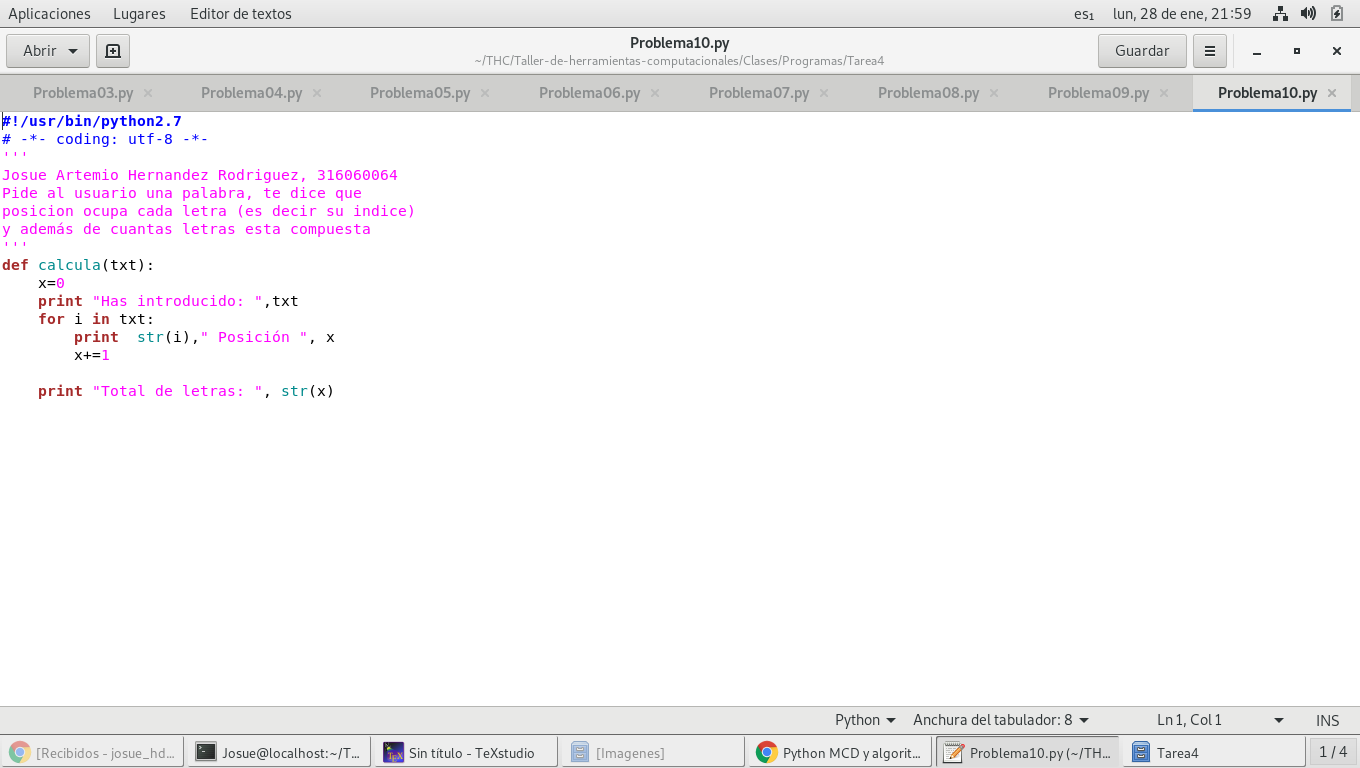
\includegraphics[scale=0.4]{pro10.png}
		
	\end{figure}

	
	
\end{document}
